% Edit this section directly. Styling is in raylo-report.sty.
\section{Categorisation performance against the providers}
The same 2,000 held-out transactions were scored several ways. Each step removes one of our layers: first the classifier, so the provider's category serves the residual; then the rules and dictionary entirely, so only the provider's own category remains, mapped through our crosswalk. The last of these is the status quo, since it is what the live model consumes.

\begin{tcolorbox}[colback=PeachTint,colframe=PeachTint,arc=3mm]
\begin{minipage}[t]{.30\linewidth}\raggedright{\color{Blue}\fontsize{26}{29}\selectfont \textbf{30\%}}\par\small Provider's own category alone, leaf level, all 2,000 rows\end{minipage}\hfill
\begin{minipage}[t]{.30\linewidth}\raggedright{\color{Blue}\fontsize{26}{29}\selectfont \textbf{74\%}}\par\small Our rules and dictionary, with the provider's category on what they miss\end{minipage}\hfill
\begin{minipage}[t]{.30\linewidth}\raggedright{\color{Blue}\fontsize{26}{29}\selectfont \textbf{83\%}}\par\small Our rules and dictionary, with our transformer classifier on what they miss\end{minipage}
\end{tcolorbox}
\begin{figure}[H]
\centering
\ChartTitle{Figure 3. The same 2,000 held-out transactions scored four ways}
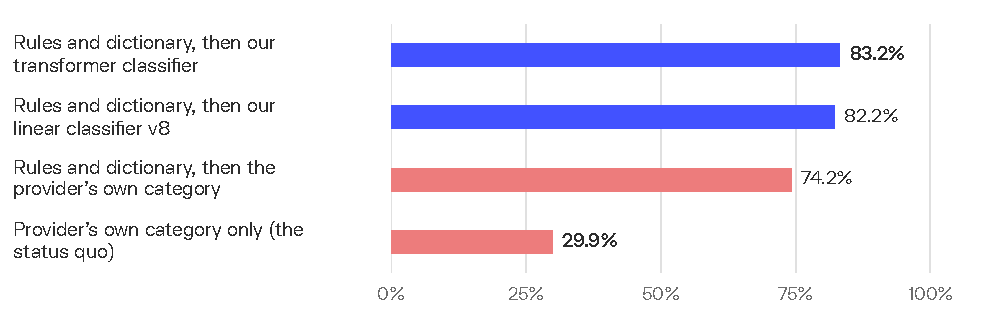
\includegraphics[width=\linewidth]{charts/fig-threeways.pdf}
\caption*{Leaf-level accuracy on the same rows. Each step down removes one of our layers. The provider's own category is what the live risk model consumes today. Rows with no provider category are counted as wrong; on provider-labelled rows alone the status quo reaches 45\%. At general level the rules-plus-classifier pipeline is 87\% and the status quo 42\%.}
\end{figure}
Where the gap comes from is worth separating. On the 1,446 rows the dictionary and early rules resolve, we are right 89\% of the time. On the Plaid rows among them where Plaid also supplies a category, we are right 92\% of the time and Plaid 32\%. Equifax is closer, at 90\% against 79\%, because its vendor field is already a curated entity and there is less for the dictionary to fix. But Equifax is a closed historical dump; live traffic is Plaid.

\begin{figure}[H]
\centering
\ChartTitle{Figure 4. Rows our dictionary and early rules resolve, where the provider also supplies a category}
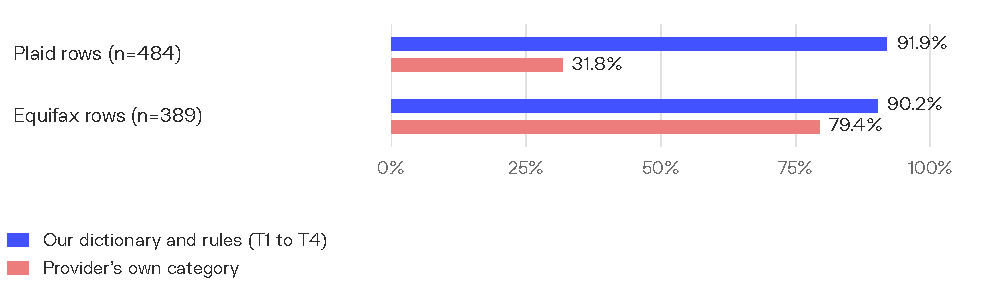
\includegraphics[width=\linewidth]{charts/fig-t14.pdf}
\caption*{Leaf-level accuracy. Plaid is where live traffic comes from and where the dictionary has most to fix; Equifax's vendor field is already a curated entity.}
\end{figure}
The residual, the 480 rows the rules cannot place, is where the machine-learning tier earns its place. There the provider's category is right 26\% of the time. Roughly half of Plaid's volume lands on coarse catch-all buckets such as "unclassified transfer", and 203 of our 275 leaves have no Plaid source at all, so categories like arranged overdraft, cash advance and pawnbroker cannot be produced from Plaid's scheme no matter how it is mapped.

\begin{figure}[H]
\centering
\ChartTitle{Figure 5. The residual: 478 rows the rules cannot place, served three ways}
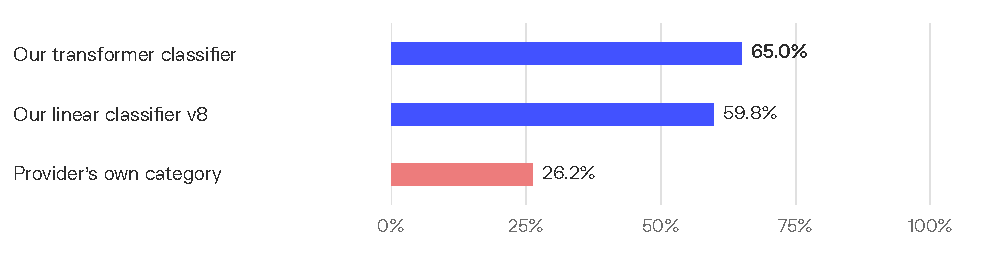
\includegraphics[width=\linewidth]{charts/fig-residual.pdf}
\caption*{This is where the machine-learning tier earns its place. Roughly half of Plaid's volume lands on catch-all buckets, and 203 of our 275 leaves have no Plaid source at all.}
\end{figure}
